\subsection{Structural modifications}

We added a sentence to the end of the abstract and introduction about the generalization of the result to smooth curves. Appendix B, following the referee's suggestion, was promoted to Section 5.

\subsection{Singularity (Remark 1)}
The concept of singularity we are using is that of parametric curves, i.e., a point $t_0$ of a smooth curve $\alpha(t)$ is called singular when $\alpha'(t_0)=0$. This definition, in general, differs from that of implicit curves $f(x,y)=0$. For example, self-intersections in parametric curves are always singularities of the implicit curve. We derived the implicit equation (as suggested by the referee) of a $\theta$-evolutoid; in general the curve is of degree 12. In several examples  it is of degree 6.
\subsection{$\theta$-evolutoid}

New redaction to Remark 1.

\textcolor{blue}{ 
\begin{remark*}
 The parametrization $[x_\theta(t), y_\theta(t)]$ of the $\theta$-evolutoid will   have 4, 2, or 0 singularities if
$\theta\in(\theta_0,\pi-\theta_0)$, $\theta\in\{\theta_0,\pi-\theta_0\}$, or $\theta\notin[\theta_0,\pi-\theta_0]$, respectively. Moreover, the ${\theta_0}$-evolutoid is singular at $t_1=\frac{3\pi}{4}$ and
	$t_2=  \frac{7\pi}{4}$.
	Here, a  point $t=t_0$ is called singular when $x'_\theta(t_0)=y'_\theta(t_0)=0$.
	These points correspond to real cusps of the curve.  
	In the implicit form,   a  $\theta$-evolutoid is given by $f^{-1}(0)$, and $f$ being a polynomial   function of degree 12.
\end{remark*}
}
\subsection{Note on page 5} We removed the note below, note it is never used in the article: (note we will use red to denote excerpts removed from the text)

\textcolor{red}{  
Note: when expressed in line coordinates, the cusps of the evolute are regular. Specifically, cusps of the evolute are inflection points of its dual % \cite{fischer2001,akopyan2007-conics}. 
}

\subsection{The equation of $\mathcal{E}_\theta$ is not given}

Inserted parametrization of $\mathcal{E}_{\theta}$ as asked. (blue means inserted)

\textcolor{blue} { 
The rotated pedal curve $\mathcal{E}_{\theta}$ is given by
$[X_\theta/\Delta,Y_\theta/\Delta]$ where:
{\small 
\begin{align*}
 X_\theta &=  - 
  \left(     {a}^{2}  \sin^2  t   
\cos^2\theta +\frac{1}{2} a b\sin \left( 2\,\theta
 \right)  \sin \left( 2\,t \right) +  b^2  \cos^2 t 
  \sin^2\theta  
 \right) {x_0} \\
&+ \frac{1}{2} \left(  (b^2
  \cos^2 t   - {a}^{2} \sin^2t)\sin \left( 2\,\theta \right)
  +ab\sin
 \left( 2\,t \right) \cos \left( 2\,\theta \right)   \right)  y_0
 \\
 &+ \frac{b}{4}(c^2 \cos t \sin(2t) + 2 a^2 \sin{ t} )\sin(2\theta) - a \cos t (b^2\cos^2\theta + c^2\, \sin^2 t\sin^2\theta) 
 \\
 Y_\theta&= \frac{1}{2} \left( (  b^2  \cos^2t -   a^2\sin ^2{t} )  \sin(2\theta)+ a b  \sin (2t)  \cos(2  \theta)       \right)  x_0\\
 &+ \left(  (    a^2 \sin ^2{t}-b^2\cos^2t) \cos^2\theta   +\frac{1}{2} a b  \sin(2\theta)     \sin(2 t)  - a^2  \sin ^2{t}\right)  y_0\\
 &+  \frac{c^2}{4}  \left(2b \cos t\sin^2\theta+ a  \sin {t}   \sin(2\theta)    \right)  \sin(2 t) 
  -\frac{ab}{2}\left(2a \cos^2\theta  \sin {t}   +b \cos{t}  \sin(2\theta)  \right)
   \\
 \Delta&={b}^{2}   \cos^2 t +{a}^{2}\sin^2t
\end{align*}
}
}

\subsection{Typo in Proposition 1}

Removed 
 \textcolor{red} {
 \[ S_{\theta}=\pi\,ab   \cos^2   \theta  -  \,{\frac {3
		    c^{2} }{8ab}}\sin^2  \theta   
\]
}
 
Inserted, changing $c^2 \rightarrow c^4$.

\textcolor{blue}{ 
\[S_{\theta}=\pi a b \cos^2\theta -\frac{  3 c^4\pi}{8 ab} \sin^2\theta\]
}

\subsection{Proposition 4: mistake in formula}

The source of the error was that calculations were done with $ \mu$ instead of $(1-\mu)$. Remove:
\textcolor{red}{\begin{align*} A_{\mu}=& \left(2\,{a}^{2}-3\,ab+2\,b^{2}+2\,x_0^{2}+2\,y_0^{2} \right) \pi\,{\mu}^2 -2\,\left( (a-b)^2  +x_0^{2}
+y_0^{2} \right) \pi\,\mu \\
+&\frac{1}{2}\left( (a-b)^2 +x_0^{2}+y_0^{2} \right) \pi\\
  =&(2\mu-1)[(1-\mu) A_p-\mu A_c]+\mu(1-\mu)A. 
\end{align*}
}

Inserted the following corrected expression:

\textcolor{blue}{ 
\begin{align*}
A_{\mu}=& \left(2\,{a}^{2}-3\,ab+2\,b^{2}+2\,x_0^{2}+2\,y_0^{2} \right) \pi\,{\mu}^2 -2\,\left( (a-b)^2  +x_0^{2}
+y_0^{2} \right) \pi\,\mu \\
+&\frac{1}{2}\left( a^2+b^2 +x_0^{2}+y_0^{2} \right) \pi\\
  =&(1-2\mu)[(1-\mu) A_p-\mu A_c]+\mu(1-\mu)A. 
\end{align*}
}

\subsection{Theorem 3: corrected the sign}
  
 \textcolor{blue}{
 	\[ A^\dagger=  -  \frac {\pi\, \left( 3\,{a}^{4}+2\,{a}^{2}{b}^{2}+3\,{b}^{4}
 \right)  \left( {a}^{2}-2\,ab-{b}^{2} \right)  \left( {a}^{2}+2\,ab-{
b}^{2} \right) }{8 a^{3} b^{3}}
	\]
 }
 \subsection{Evolutoids}
 Referee says: ``An additional mistake must have happened in the equations for the evolutoids''. Solution: there is a typo in the equation of the family $\mathcal{L}_{\theta}(t)$ (below, removed)

\textcolor{red}{ 
\begin{align*} 
\mathcal{L}_{\theta}(t):& \left( \sin \left( 2\,\theta \right) +\sin \left( 2\,t \right) 
\right) x+ \left( \cos \left( 2\,\theta \right) -\cos \left( 2\,t
\right)  \right) y\\
-&h(t)  (  \sin t - 
 \sin \left( 2\,\theta+t \right) )+  h '(t)   (  \cos t -\cos
\left( 2\,\theta+t \right) )=0
\end{align*}
}

Inserted the following correction (blue below):   

In the report, we think that the referee computed with angle $-\theta$. This is a choice of orientation.  See Fig. below.

 The equation \eqref{eq:line-theta} can be simplified as:
\textcolor{blue}{
\[ 
 \mathcal{L}_{\theta}(t):   \cos(\theta-t) \,x -  \sin(\theta-t)\, y - h(t) \cos\theta + h'(t)  \sin\theta = 0 \]
 }

Therefore we think we should maintain the two expressions below as in the original (see Figure~\ref{fig:referee}. Let $\mathcal{C}_\theta(t)=(x_\theta,y_\theta)$ denote the envelope of $\mathcal{L}_\theta(t)$. This will be given by:
 
\begin{align*} x_{\theta}(t)=&\frac{1}{2}  \left( \cos \left( t-2\,\theta \right) + 
  \,\cos t  \right) h \left( t \right) -h'(t)\sin t    +\frac{1}{2} \left(\cos \left( t-2\,\theta 
  \right) - \,\cos t  \right)  h'' \left( t \right) \\
  %
  y_{\theta}(t)=&\frac{1}{2} \left(\sin \left( t-2\,\theta \right)  +
  \,\sin t \right) h(t)   +h'(t)\cos t    +\frac{1}{2} \left(\sin \left( t-2\,\theta 
  \right) - \,\sin t  \right)  h'' (t)
 \end{align*}
 
  

 \begin{figure}[H]
     \centering
     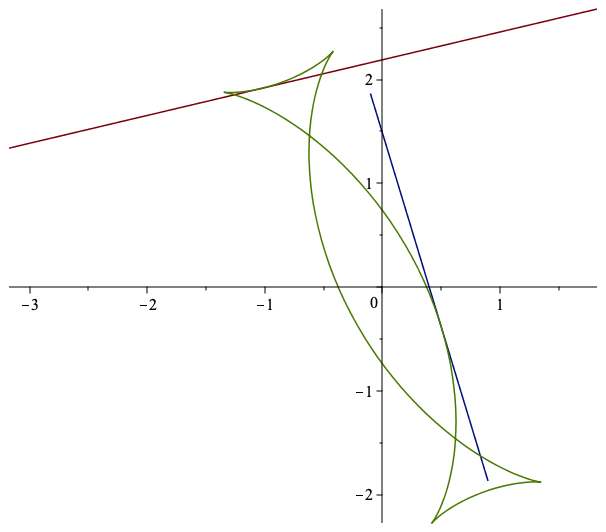
\includegraphics[scale=0.5]{pics/figura_gerada_curva_referee.png}
     \caption{Curve produced with  $\theta=-\pi/3$ and lines with $t=\pi/4$ (red) and $t=-\pi/4$ (blue). Support function $h(t)=2\cos^2(t) + 3\sin^2(t)$ as in the report. The curve was drawn taking into account  the correction of a typo in equation of $\mathcal{L}_{\theta}$. Note our $\theta$ is equal to $-\theta$ of referee's equations obtained in the report.}
     \label{fig:referee}
 \end{figure}
 
 %\textcolor{blue}{ reconferi calculos e esta ok essa equacao acima.
 %
 %}
 

 \subsection{ Negative pedal curve}
 
 %$\bullet $  {\bf Negative pedal curve}
 
Recall $\mathcal{E}^\dagger$ is the negative pedal curve of $\mathcal{E}^*$ (Section~\ref{sec:intro} and Figure~\ref{fig:hybrid-npc}). For $M=[a\cos u,b\sin u]$ on the ellipse, the coordinates $[x^\dagger,y^\dagger]$ of $\mathcal{E}^\dagger$ can be derived explicitly. Recall the original equation (below):
\textcolor{red}{{\small
\begin{align*}
x^{\dagger}(u)=&-{\frac { \left( \left(  k_x+1 \right) {a}^{4}-2
 \left(k_x+1\right) {b}^{2}{a}^{2}+ k_x b^4  \right)\cos u
}{{b}^{2}a}}\\
-&2\,{\frac { \left( {a}^{2}-{b}^{2} \right) ^{2}   
\sin^{3}t \cos{t}\sin{u}}{{b}^{2}a}} 
 + \frac {\cos t \left( {a}^{2}+{b
}^{2} \right)  \left( -{a}^{2} \sin^2t-{b}^{2} \cos^2t+2\,{b}^{2}
 \right) }{{b}^{2}a}\\
 y^{\dagger}(u)=&-2\,{\frac { \left( {a}^{2}-{b}^{2} \right) ^{2}\sin t
 \cos^3{t}  \cos u}{{a}
^{2}b}}-{\frac { \left(  \left(k_y-1 \right) {a
}^{4}-2 k_y {b}^{2}{a}^{2}+
 k_y {b}^{4} \right) \sin u}{{a}^{2}b}}\\
 +&{\frac {\sin t \left( {a}^{2}+{b
}^{2} \right)  \left( ({a}^{2}-b^2) \cos^2t+{a}^{2} \right) 
}{{a}^{2}b}}\\
k_x=&2\cos^4t-3\, \cos^2t\\
k_y=&2\cos^{4}t- \cos^2t
\end{align*}
}
}

We have replaced the above by the following simplified expression

\textcolor{blue}
{\small  
\begin{align*}
x^{\dagger}(u)=&\frac{\left(c^4(2\cos(2t) - \cos(4t)) - (a^2 - 3b^2)(a^2 + b^2)\right)\cos{u} }{4 a b^2} - \frac{2c^4 \sin^3t \cos{t} \sin{u}}{a b^2}\\
&+ \frac{(a^2 + b^2)(b^2-c^2\sin^2{t}  )\cos{t}}{a b^2}\\
y^{\dagger}(u)=&-\frac{2c^4 \sin{t} \cos^3{t}\cos{u}}{a^2b} - \frac{(c^4(2\cos(2t) + \cos(4t)) - (3a^2 - b^2)(a^2 + b^2))\sin{u}}{ 4a^2b}\\
&+\frac{  (a^2 + b^2)(c^2 \cos^2{t}    + a^2)\sin{t}}{a^2 b}
\end{align*}
}
\subsection{Comments about Proposition 9 (originally in App B)}
  
First of all it was moved with the appendix to section 5. It is now Proposition 7. It is derived using the parametrization by the support function. Note the change of $2 \mu-1 \rightarrow  1-2\mu$. Now it reads>
 
 \textcolor{blue}{\textbf{Proposition 7}: For any smooth regular closed curve $\mathcal{C}$ with non-zero rotating index, the isocurves of $A(\mathcal{C}_\mu)$ are circles centered on $K$.
In fact, \[A(\mathcal{C}_\mu) =(1-2\mu)[(1-\mu) A(P_M)-\mu A(C_M)]+\mu(1-\mu)A(\mathcal{C}).\] 
 }

\subsection{Example 1 }
An example was introduced to better explain Fig. 11. An update of the   Figure  and a video were produced. Also added two video links at the end of the figure's caption which illustrate continuous interpolation and area invariance over a circle centered on K. The curve used in the example is shown here for reference in Figure~\ref{fig:convex-curve}, here is a copuy of the example already in the text:

\textcolor{blue}{
  Consider the non convex smooth curve 
\[ 
\mathcal{C}(t)= [  2 \cos t -\frac{1}{4}\sin( 2t) + \frac{3}{10}\cos(2t),
\sin{t} + \frac{3}{4}\cos(2t)] \] 
The curvature centroid of $\mathcal{C}$ is $K=[0.1823\ldots, 0.01943\ldots]$. The  centroid
$[\int xds/\int ds, \int yds/\int ds]$ is the point $[0.1387\ldots, -0.2504\ldots ] $ and the center of mass $[\int xdxdy/\int dxdy, \int ydxdy/\int dxdy]$ is $[12/95, 7/19]=[0.1263\ldots, -0.3684\ldots]$.
}

   \begin{figure}[H]
       \centering
   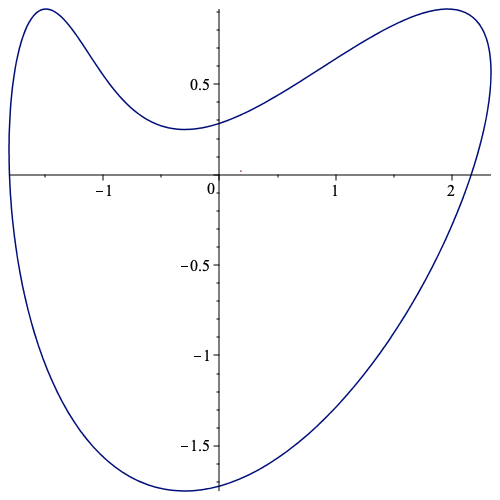
\includegraphics[scale=0.3]{pics/figura11.png}
       \caption{Non convex curve with curvature centroid  $K=[0.1823\ldots, 0.01943\ldots]$.}
       \label{fig:convex-curve}
   \end{figure}


\subsection{Corollary 6} The proof of Corollary 6 was reformulated and a remark for convex curves was added.


\textcolor{blue}{\textbf{Corollary 6} The family of isocurves of $A(P_M)$ and $A(C_M)$ are circles centered at
\begin{align*}
\label{eq:centroK}
K_0=\left[	\frac{1}{\pi} \int_0^{2\pi}\!\!\!\!\! h(t)\cos t \,dt,	\frac{1}{\pi} \int_0^{2\pi}\!\!\!\!\! h(t)\sin t \, dt\right]
\end{align*}
}

\textcolor{blue}{\begin{proof}  Consider the mean $K_0=\frac{1}{2\pi}\int_0^{2\pi}\mathcal{C}(t)dt$ of the curve $\mathcal{C}$ given by Equation \eqref{eqn:support}. Integration by parts leads to the result stated. Expressions of the areas $A(P_M)$ and $A(C_M)$ given in Equation \eqref{eqn:apm-acm} shows that the isocurves are cirles centered at $K_0$.
\end{proof}
}

We also added the following remark

\textcolor{blue}{\textbf{Remark: } For convex curves,  $K_0$ coincides with the   centroid of Steiner $K$ given by Equation \eqref{eqn:steiner-k}. In fact, using the parametrization  of the curve $\mathcal{C}$ given by Equation \eqref{eqn:support} it follows that $ds= |h(t)+h''(t)|dt$ and $k(t)=1/(h(t)+h''(t))$. Integration by parts leads to the result.}
